\chapter{Metode}
Dette afsnit vil beskrive de anvendte metoder til udarbejdelsen af denne rapport. Hvorfor disse metoder er blevet anvendt og hvilket formål de har haft vil blive beskrevet, samt hvilke tanker der hat lagt til grund for dette igennem problemanalysen og problemløsningsafsnittet. Læseren kan med fordel se tilbage til dette afsnit, for at forstå hvordan der er blevet arbejdet igennem forløbet, skulle der opstå tvivl over hvordan vi er nået frem til vores deduktioner og resultater.

\section{Problemområde}
Problemområdet er det som danner grundlaget for projektet. Det har til formål at give et overblik over hvilke aspekter det valgte problem belyser, ud fra den initierende problem. Det klarelægger hvem problemet påvirker og hvem det vil gavne såfremt en løsning på problemet kan opnås til at analysere både problemets relevans og samt om det har nogle interessenter.  Ud fra det initierende problem er der blevet stillet følgende hv-spørgsmål til at afgrænse problemets omfang;

\begin{figure}[H]
\begin{adjustbox}{width=1.2\textwidth,center=\textwidth}
\centering
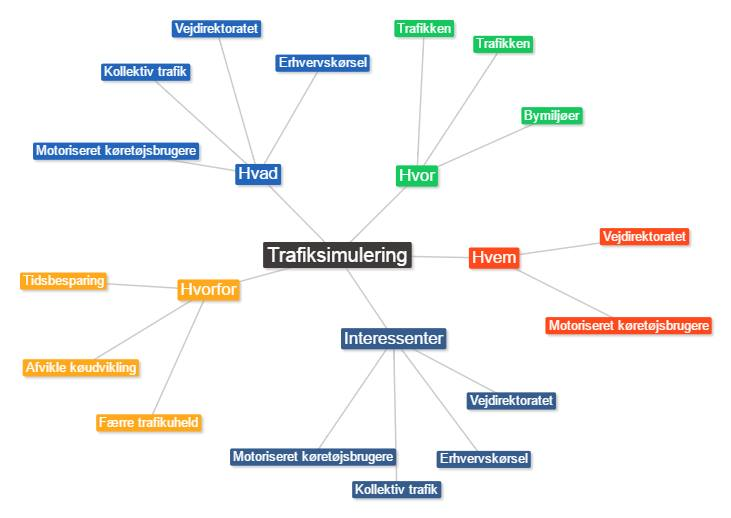
\includegraphics[width=1.2\textwidth]{Pictures/Metode/metodebillede.jpg}
\end{adjustbox}
\label{fig:problemtreae}
\caption{Problemtræ over trafiksimulering}
\end{figure}

\begin{itemize}
\item Hvorfor: Hvad er årsagerne til problemet?
\item Hvad: Hvem bliver ramt af problemet?
\item Interessenter: Hvem er interessenterne - hvem har en interesse i en løsning på problemet?
\item Hvor: Hvor findes problemet?
\item Hvem: Hvem er hovedpersonerne i problemet?
\item Hvordan: Hvordan kan problemet løses?
\end{itemize}
men også for at finde ud af at hvorvidt det opstillet problem har nogen relevans for at blive afviklet. Problemområdet er således blevet benyttet til at isolere alle de relevante aspekter af problemet, hvorefter det er blevet sat sammen i en større sammenhæng for at give et klart og tydeligt billede af hvor det præcise problem befinder sig til at udarbejde en problemformulering.

\section{Fremgangsmåde}
Under udarbejdelse af projektet er der blevet benyttet flere forskellige fremgangsmåder, alt efter hvad der er blevet arbejdet med under problemanalysen. Fremgangsmåden under udarbejdelsen af rapporten er foregået ved at opstille relevante hypoteser, som enten kunne be- eller afkræftes ved at researche sig frem til eller ved hjælp af en prøve-fejl-metode.

\subsection{Emperiske-induktive-metode}
Under problemanalysen er den emperiske-induktive-metode blevet anvendt til at sikre os, at den information der er blevet indsamlet har statistisk belæg for deres udsagn eller er matematisk bevist. Dette gøre det muligt at udlede logiske slutninger til at underbygge rapportens argumentation, og sikre at troværdigheden i det som er blevet formidlet.

\subsection{Andre metoder}
Her tilføjes det hvis vi i løbet af rapporten anvender andre metoder. 

\subsection{Prøve-fejl-metoden}
Under programmeringsfasen er der hovedsageligt blevet anvendt prøve-fejl-metoden, eftersom det har været den mest effektive metode til at opnå den ønskede effekt i programmet. Dette er blevet gjort ved at lave metoder, med et specifikt mål i tankerne til at udføre bestemte dele. Hvis metoden ikke opførte sig som forventede blevet den omprogrammeret, indtil den bestemte metode udførte den ønskede effekt i programmet.
%http://kom.aau.dk/~dsp/ComSys08/ComSys07/sites/ComSys6/4%20Videnskabelige%20metoder.pdf 

\section{Kildekritik}
For at finde frem til relevant information, er der blevet taget udgangspunkt i kilder med ophav fra statslige instanser eller anerkendte virksomheder og organisationer, for at sikre informationernes gyldighed og troværdighed. Dette vil det også være muligt at kunne kontakte kilderne for uddybende spørgsmål, skulle der opstå tvivl om dele af informationen eller indsamlet data i det anvendte information. Ydermere er der blevet forsøgt at finde den nyeste tilgængelige information, for at sikre at den indsamlede data stadigvæk er brugbart og gyldigt. Fordi flere af de anvendte kilder kunne have en tendens, er den præsenteret information blevet kritisk overvejet efter hvorvidt det forholder sig objektivt eller om det er blevet fremstillet til at opnå noget for egen vinding eller et specielt mål.

\end{itemize}
 Den anvendte information er så vidt muligt også forsøgt at krydsrefereret med andre tilsvarende kilder, for at øge troværdigheden ved at undersøge om andre er nået frem til tilsvarende konklusioner og data.
